\section{Methods}
One of the most common problems in inferring knowledge from data is approximating difficult to compute or intractable posterior probability densities. Markov Chain Monte Carlo sampling techniques are one of the most common and traditional methods to tackle such problems \cite{Hastings1970}. Another clever alternative to estimate hard to compute probability distributions is a Machine Learning technique called Variational Inference (VI) (\cite{Hoffman2013}). VI has been applied to many different applications and it tends to be faster than sampling methods. VI formulates the posterior estimation problem as an optimization problem over a family of distributions. To get an essence of the same, let's consider a set of observed data $\vx$, and latent variables $\vz$ underlying the observed data. 

\subsection{Variational Inference and Variational Autoencoders}

In most general setting of a bayesian model, the latent variables govern the data distribution i.e. a generative process draws the latent variables from some prior distribution $p(\vz)$ and generates the observed data through a likelihood $p(\vx|\vz)$. Our target is to learn about $\vz$ given the observed $\vx$, which is governed simply by the Bayes' rule:
\begin{align*}
 p( \vz | \vx)&= \frac{p(\vx|\vz)p(\vz)}{\int_z p(\vx|\vz)p(\vz) dz} \numberthis \label{bayes-rule}
\end{align*}
The denominator can be intractable, making it difficult to estimate $p( \vz | \vx)$.  VI starts off with assuming that the posterior can be approximated by a distribution $q(\vz)$ from the family $\cQ$ and formulates the following optimization problem which minimizes the KL divergence between approximator and the true posterior. 
\begin{align*}
 q^*(\vz) &= argmin_{q(\vz)\in\cQ} KL(q(\vz)||p(\vz|\vx)) \numberthis \label{vi-formulation}
\end{align*}
There are certain properties that this inference technique gives to the estimated posterior. We would like to point out one of them. If $p(\vz|\vx) \rightarrow 0 $ for some $\vz$, then the optimization results in $q^*(\vz) \rightarrow 0$. This can result in underpredicted variance if we are not careful about the choice of the distribution family $\cQ$. A simple example is if $p(\vz|\vx)$ is bimodal with a very low probability region between the modes and $q(\vz)$ is unimodal. VI will estimate one of the mode and  completely ignore the other one in that case.

There has been extensive work in forming various strategies to solve the VI optimization problem in various settings e.g. \cite{Zhang2019}, \cite{Ingraham2017}, \cite{Bouchard-Cote2010}. It should be noted that VI is essentially solving an optimization problem over function families and neural networks are extremely popular candidates for representing and learning complex functions. \cite{Kingma2014} incorporated the idea of VI into the AutoEncoder framework and came up with the architecture of Variational AutoEncoders (VAE)  .  VAE essentialy consists of an encoder network encoding the   function $q_\vx(\vz)$ approximating $p(\vz|\vx)$, and a decoder network $p(\vx|\vz)$. The idea is to encode each input point $\vx_i$ as a distribution over a latent space $\vz$ with some prior distribution over $\vz$ and also project $\vx_i$ to a point $\vz_i$ using the reparametrization trick (\cite{Kingma2014}). Traditionally, VAEs use the standard  normal prior $\cN(0,\vI)$ as the prior distribution over the latent space. The decoder network takes points from the latent space ($\vz$) as input and generates ($\vx$) i.e. the decoder simulates the generative process of the input $p(\vx|\vz)$ from the latent variables, while the encoder does the job of modelling the posterior distribution $p(\vz|\vx)$ as some $q^*_\vx(\vz)$.  Commonly, VAEs model the posterior distribution as a multidimensional spherical Gaussian $\cN(\mathbf{\mu},\mathbf{\Sigma})$ with same dimensionality as $\vz$.  

Training a VAE then essentially reduces to minimising the following  two objectives:
\begin{enumerate}

 
 \item  The encoder network should learn a ``well distributed'' latent space which can be ensured by minimising the KL divergence $KL(\cN(\mathbf{\mu},\mathbf{\Sigma}) || \cN(0,\vI)) $.
 \item An input $\vx$ should be meaningfully reconstructed by the network at the end of learning. This can be ensured by either by an additional $L1$ or $L2$ loss function $|\vx - \hat{\vx}|$ or $(\vx - \hat{\vx})^2$ where $\hat{\vx}$ is the output of the decoder. 
\end{enumerate}
It can be shown that the VAE architecture trained using the above KL-loss and $L2$-reconstruction loss, solves the VI formulation described in \eqref{vi-formulation}. However, other variations of the reconstruction loss can be used in practice to tackle practical challenges. For example, $L1$ loss can be preferred over $L2$ when we don't want outlier points to influence the $\vz$ structure too much, because $L2$ error is known to be susceptible to outliers (\cite{botchkarev2018performance}).
%here \eqref{eqn}
\subsection{Recurrent Variational Autoencoder for gene expression dynamics (RVAgene)}
So far, we haven't specified anything about architecture of the encoder and decoder networks of a VAE, except that they learn certain functions modelling the posterior and likelihood probabilities  of our generative story of the data we are interested in. In general we could make them a fully connected neural network. But, since we are interested in handling sequential (time-series) data, we expect a specific structure of those functions. Intuitively, the $t$-th time point of input sequenece $\vx$ should be causally dependent only on its previous timepoints (upto $t-1$).  Therefore, instead of designing a completely agnostic network (e.g. fully connected layers), we can use a recurrent architecture for the encoder and decoder, which are well established in modelling sequence data (e.g. text data (\cite{Nallapati2016}), time-series data (\cite{Malhotra2015})). This in essence reduces the search space of the model from completely agnostic to a family of recurrent functions.

\begin{center}

% 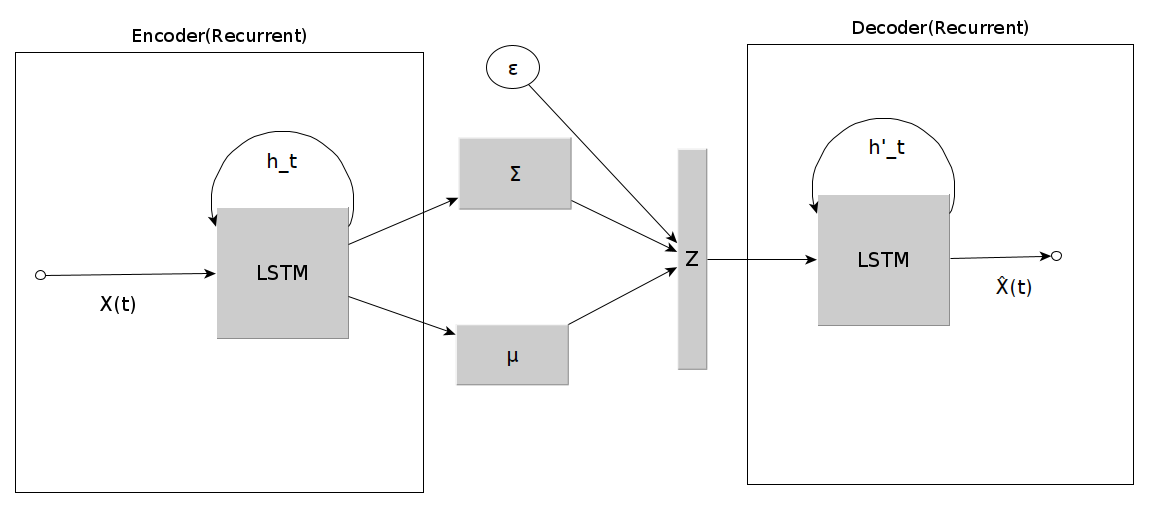
\includegraphics[scale=0.3]{architecture.png} 
\begin{figure}[h]
\centering
  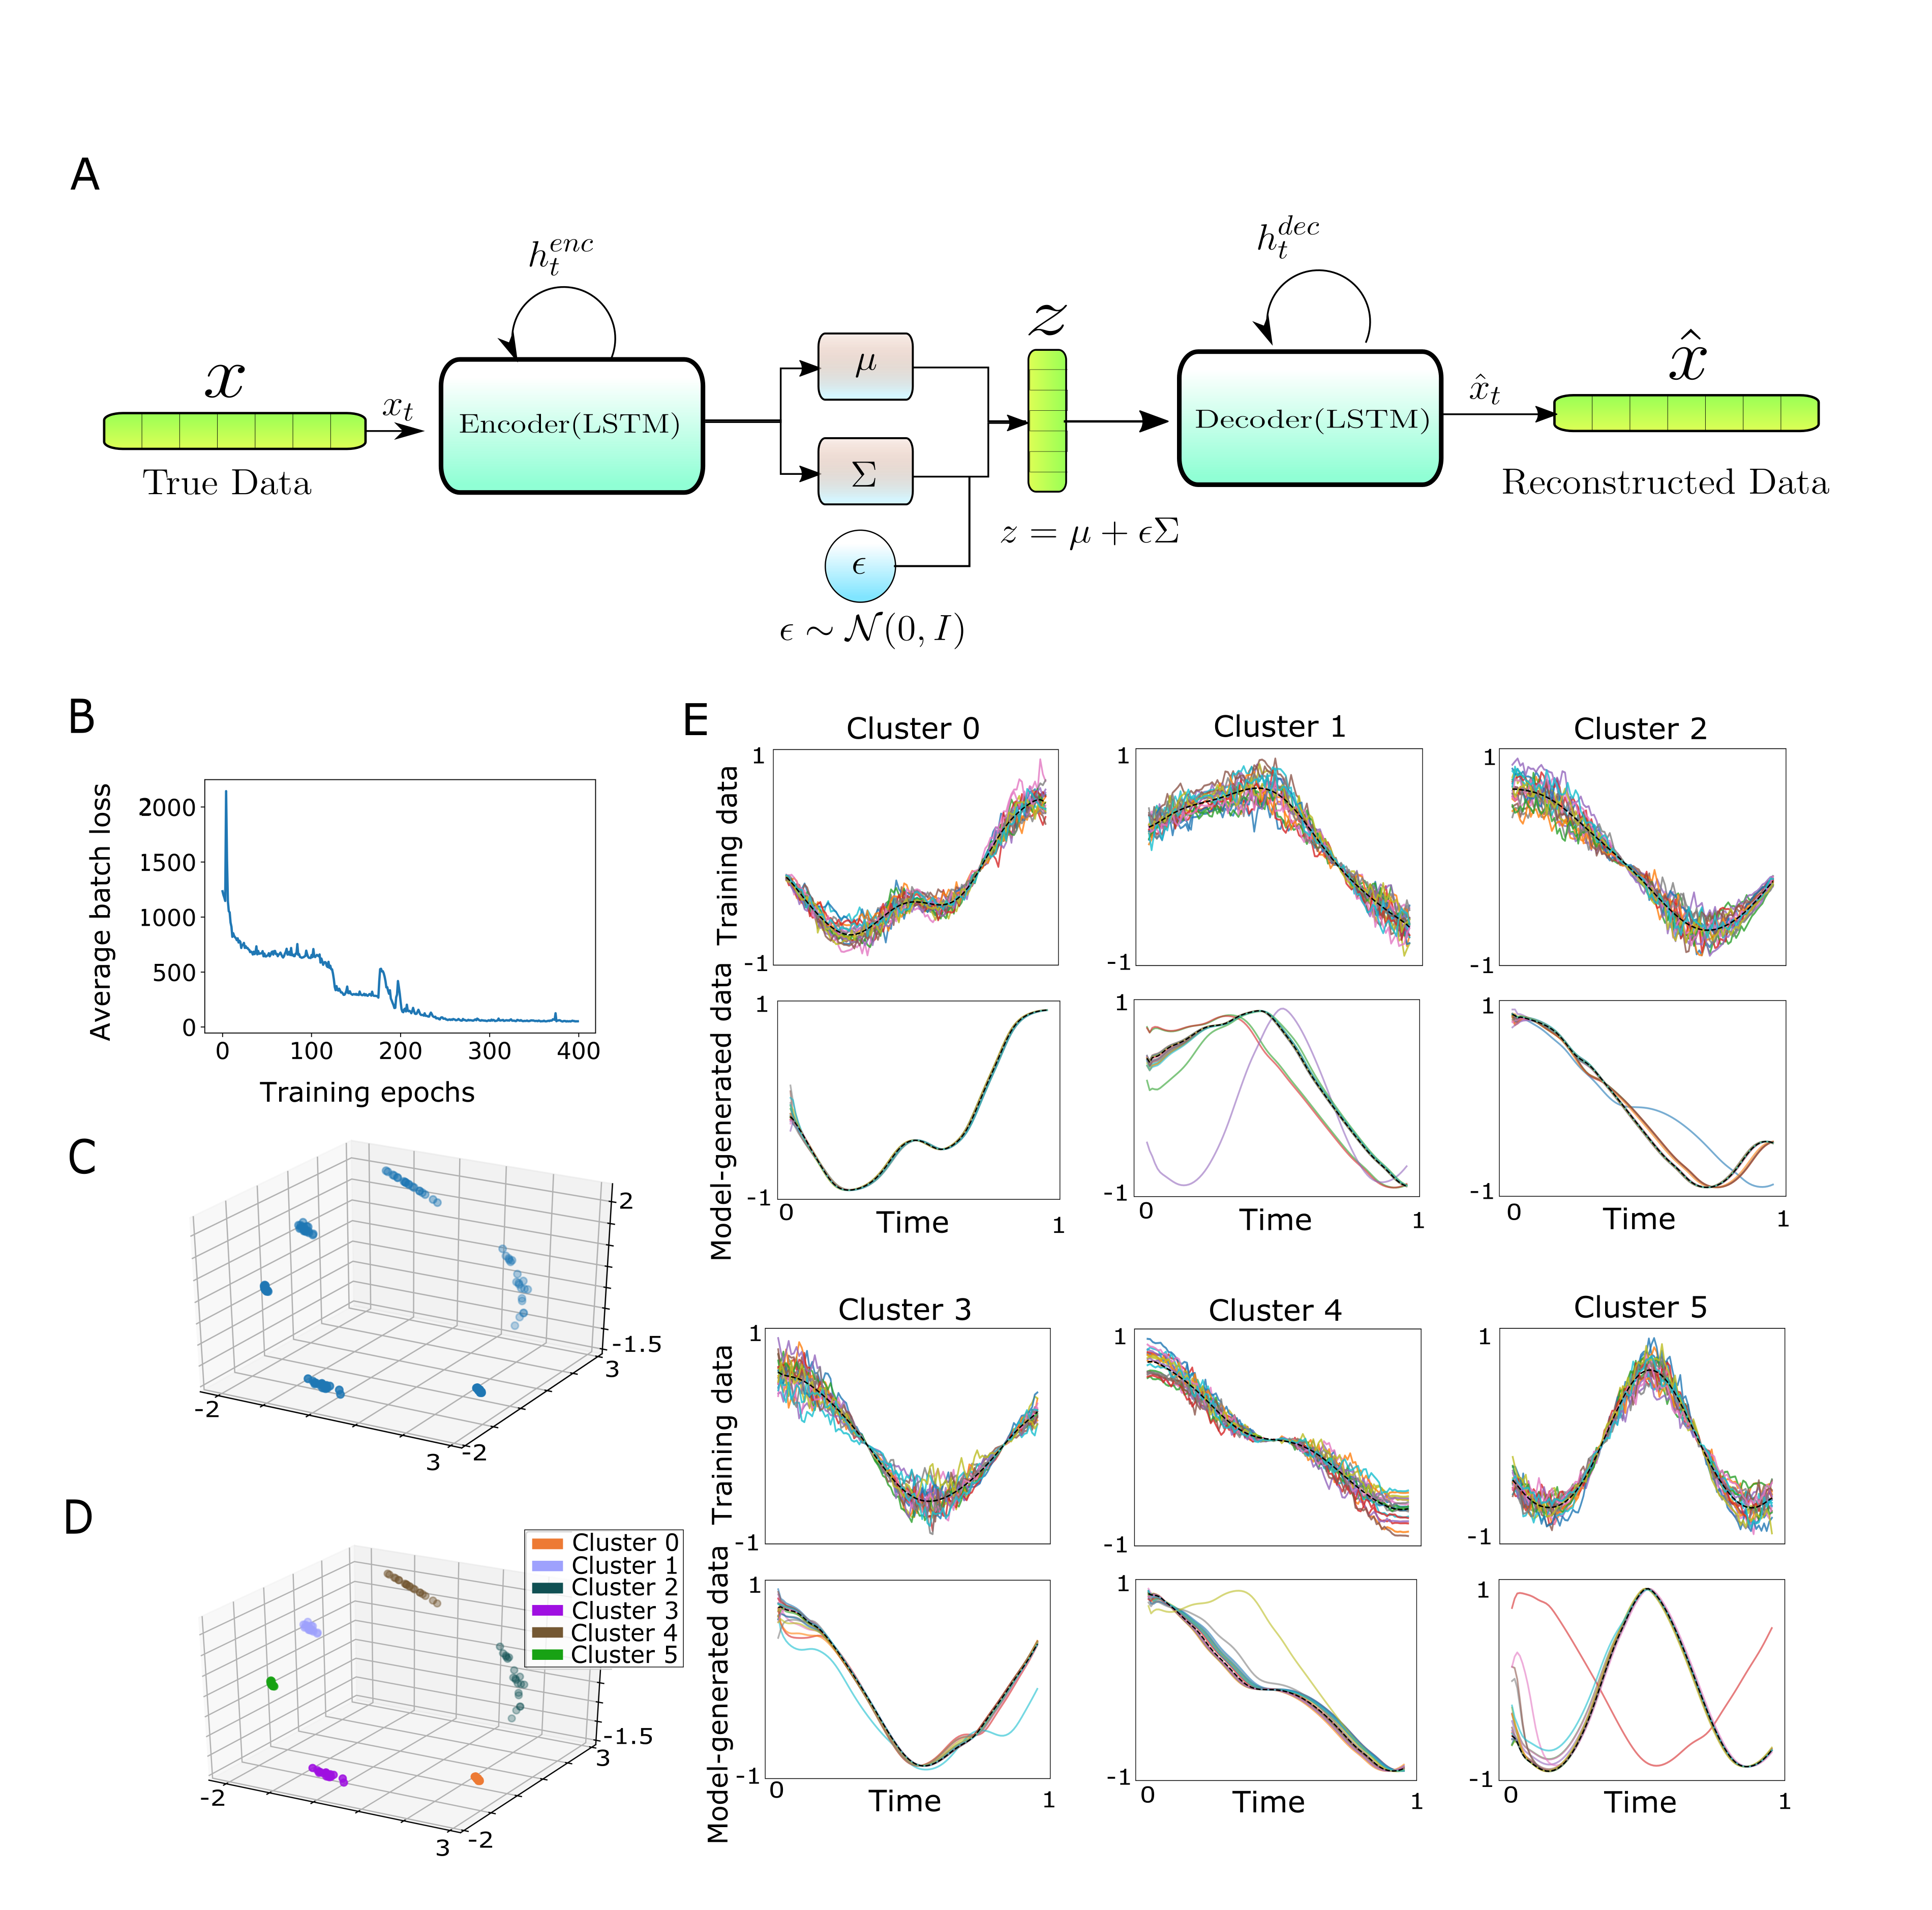
\includegraphics[width=\linewidth]{figures/fig1.png}
 % archetecture.png: 1149x508 px, 72dpi, 40.53x17.92 cm, bb=0 0 1149 508
 \caption{Schematic diagram of RVAgene.}
 \label{fig:scheme}
\end{figure}


\end{center}

\cite{Fabius2015} used this idea and showed how Recurrent Variational Autoencoders can be
 useful as a unsupervised latent representation learning and generative model for
music data. 

Next, we present the architecture of RVAE based on \cite{Fabius2015} and modified according to our convenience.  Let, the encoder network has parameters $W_{enc}$, $W_{inp}$ and a bias term $b_{enc}$, the input sequence $x = (x_1,x_2,x_3,...,x_t,...x_T)$ gets encoded using a recurrent function  described by an LSTM unit. LSTM units are state of the art recurrent architectures which are robust against vanishing gradient problem for longer sequences that traditional recurrent units suffer. We shall avoid  full details of LSTM units which can be found in \cite{Hochreiter1997}. Therefore, we encode x in the following manner:
\begin{align*}
 h_{t+1} &= LSTM(W_{enc}^Th_t + W_{inp}^T{x_t}+b_{enc}) \numberthis \label{lstm}
\end{align*}
\green{The parameters $h^t$ are called hidden states and they represent information shared over timepoints in the LSTM. Dimensionality of $h^t$ is a hyperparamter to the model named "hidden-size".} Next we take the encoded $h_{t+1}$ and parametrize it to posterior mean and variance for $x$.
\begin{align*}
 \mu_z &= W_{\mu}^Th_T + b_{\mu} \numberthis \label{mu}\\
  log(\sigma_z) &= W_{\sigma}^Th_T + b_{\sigma} \numberthis \label{sigma}
\end{align*}
Now, we can use the reparametrization trick as described in \cite{Kingma2014} to sample z from this distribution:
\begin{align*}
 z = \mu_z + \epsilon\sigma_z \numberthis 
\end{align*}
Note, the above reparametrization with a known $\epsilon$ makes backpropagating through the sampling step possible while training the network. Now, for the decoder, the first state $h_0$ is calculated using $z$ and the recurrent formulation follows in reconstructing $x$ as $\hat{x} = (\hat{x}_1,\hat{x}_2,...,\hat{x}_t,...,\hat{x}_T )$.
\begin{align*}
 h_0 &= sigm(W_{z}^Tz + b_{z}) \numberthis  \\
h_{t+1} &= LSTM(W_{dec}^Th_t + W_{out}^T{\hat{x}_t}+b_{dec}) \numberthis \label{decoder_lstm} \\
\hat{x}_t &= sigm(W_{out}^Th_t + b_{out}) \numberthis
\end{align*}
Figure \ref{fig:scheme} shows a simplified schematic diagram of the whole network which can now be trained using backpropagation to minimize the following loss function: 
\begin{align*}
 \cL(\theta,\vx^i) = D_{KL}(\cN(\mathbf{\mu}|\mathbf{\Sigma})||\cN(\mathbf{0},\vI)) + |\vx^i - \hat{\vx}^i| \numberthis \label{lossfunction}
\end{align*}
\subsection{Quantifying reconstruction error}
To evaluate how good a reconstruction generated by RVAgene is, we need a good error measure. For a test gene, we calculate L1 reconstruction error averaged over all time points  after scaling them to the 0-1 range to prevent expression magnitudes skewing the error measure. Mathematically, $ \frac{1}{T}\sum_{t}|scaled(\hat{\vx})_t - scaled(\vx)_t| $.
\subsection{Generating synthetic temporal gene expression data} To demonstrate  essential workings of RVAgene, we performed experiments on simulated gene expression time series data. We generated 6 clusters of genes with 20 genes per cluster. For each cluster $c$ a mean gene expression $Y_c = (y_{c1},y_{c2},..,y_{ct})$ was generated using addition or convolution of two random sinusoidal functions. Individual cluster members were generated by drawing from the multivariate normal $\cN(Y_c,\Sigma_c)$ where $\Sigma_c$ can be modeled by the positive definite matrix $\alpha Y_cY_c^T$ where $\alpha$ is a scaling factor. $\alpha = \frac{1}{|Y_c Y_c^T|}$ is a reasonable normalising choice. $\Sigma_c$ modeled as above captures some correlation for all pairs of time points $(t_i,t_j)$. But, we probably do not want that. We can set to 0 the entries of $\Sigma_c$ for which column and row indices have a difference of more than some threshold $T$. Note, this does not necessarily keep the matrix positive definite anymore. Samplers implemented in standard python libraries can still sample using this augmented $\Sigma_c$ while introducing some noise to the individual genes, reflecting the fact that the correlation information between some time point pairs is lost in the generating multivariate Gaussian, which is welcome in the sense that it makes the simulated genes more realistic. 

